\documentclass[12pt,a4paper]{report}
\usepackage[utf8]{inputenc}
\usepackage[T1]{fontenc}
\usepackage[french]{babel}
\usepackage{geometry}
\usepackage{graphicx}
\usepackage{hyperref}
\usepackage{setspace}
\usepackage{titlesec}

\geometry{margin=2.5cm}
\setstretch{1.3}
\hypersetup{
    colorlinks=true,
    linkcolor=blue,
    urlcolor=blue
}

\titleformat{\chapter}[display]
{\normalfont\huge\bfseries}{\thechapter}{20pt}{\Huge}

\begin{document}

% =====================
% PAGE DE GARDE
\begin{titlepage}
\centering
{\Huge\bfseries Rapport de stage \par}
\vspace{1cm}
{\Large Développeur web front-end \par}
\vspace{1cm}
{\Large Office des Postes et Télécommunications (OPT-NC) \par}
\vfill
\textbf{Réalisé par :} Quoc-Kim BUI \\
\textbf{Période :} 01/07/2025 – 01/09/2025 \\
\textbf{Lieu :} Nouméa, Nouvelle-Calédonie
\vfill

\includegraphics[width=0.3\textwidth]{ressources_rapport/logo_opt.jpg}
\vfill
\textbf{Maître de stage :} Adrien SALES \\
\textbf{Professeur tuteur :} Loïc SALMON
\end{titlepage}

% =====================
% RÉSUMÉ FR + ABSTRACT EN
\chapter*{Résumé}
\addcontentsline{toc}{chapter}{Résumé}

\section*{Résumé}
Ce rapport retrace les deux mois de stage effectués au sein de la section GLIA (Génie Logiciel Inter-Applicatif) de l’OPT-NC en tant que développeur web front-end.  
L’objectif principal était la refonte de l’application \textit{"L’OPT près de chez moi"} pour la rendre plus moderne, ergonomique et adaptée aux usages mobiles.  
Après une prise en main rapide des technologies Next.js, React et Leaflet, une première version a été développée puis améliorée en fonction des retours internes.  
Les résultats sont positifs : l’application est plus performante, intuitive et maintenable.  
Des perspectives d’évolution existent, notamment un temps de trajet estimé de l'agence selectionnée pour chaque mode de transport, ou même un mode hors-ligne pour les zones à faible couverture.

\vspace{1cm}
\textit{Mots-clefs : application web, OPT, Next.js, recherche agence}

\newpage

% =====================
% TABLE DES MATIÈRES
\tableofcontents
\newpage

% =====================
\chapter{Introduction}
\section{Contexte du stage}
J'ai décidé d'effectuer un stage de deux mois en développement web front-end au sein de la direction des systèmes d’information de l’OPT-NC. Ce stage avait pour objectif principal de contribuer à la modernisation d’une application web interne et publique : \textit{\href{https://www.opt.nc/service/l-opt-pres-de-chez-moi-trouver-une-agence}{"L'OPT près de chez moi, trouver une agence"}}.

\vspace{1cm}
Avant de m'intéresser à ce stage, j'avais auparavant contacté OPEN-NC (cluster des entreprises du développement numérique) début avril dans l'optique de faire un stage dans le développement web pour mettre en avant mes compétences dans ce domaine qui ont été forgées grâce à mon DUT MMI et ma Licence MIAGE. OPEN-NC a bel et bien partagé ma demande de recherche de stage à ses entreprises partenaires (plus de 90 entreprises), mais sans succès car je n'ai eu aucune réponse de leur part.

\vspace{1cm}
J'ai donc signalé ma difficulté à trouver un stage à l'équipe pédagogique de la licence MIAGE. M. Loïc SALMON m'a répondu qu'il avait un contact de l'OPT qui pourrait prendre des stagiaires : M. Adrien SALES. Par conséquent, je lui avais directement envoyé mon CV et il m'a pris en tant que stagiaire en développement web front-end.

\vspace{1cm}
Mon stage était d'une durée de 8 semaines, du 1er Juillet 2025 jusqu'au 1er Septembre 2025. Il a été réalisé en distanciel car manque de poste sur place, donc on a utilisé LinkedIn et GitHub pour communiquer.


\section{L'OPT en bref}
\cite{blog_opt} L’Office des Postes et Télécommunications de Nouvelle-Calédonie (OPT-NC) est un établissement public à caractère industriel et commercial fondé en décembre 1956, puis mis en service le 1er janvier 1958. C'est l’acteur principal des services postaux, bancaires et télécoms sur le territoire calédonien. Fort de son statut de monopôle sur certaines activités stratégiques, il joue un rôle essentiel dans la gestion et l'entretien du réseau calédonien.

\vspace{1cm}

\begin{figure}[h] % h = here (placer l'image ici)
    \centering
    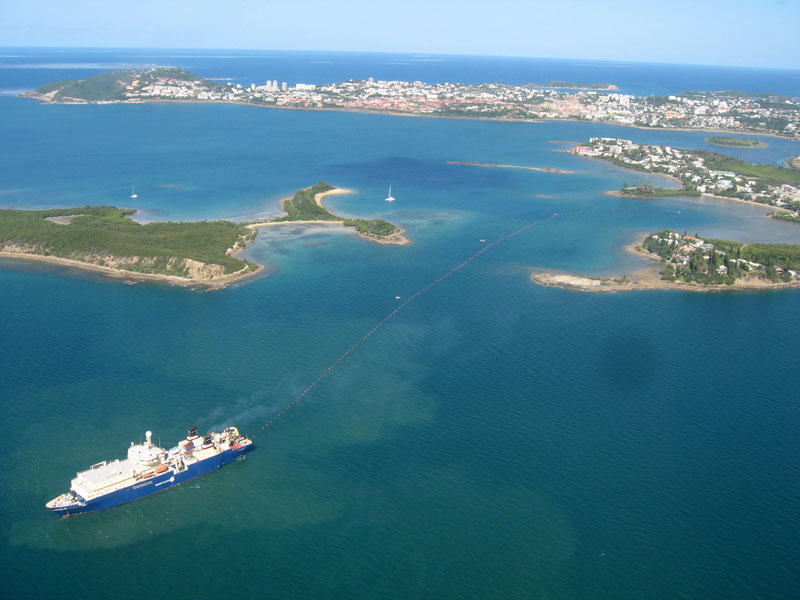
\includegraphics[width=0.7\textwidth]{ressources_rapport/pose-cable-gondwana.jpg}
    \caption{Posage du premier câble à fibres optiques sous-marin international - GONDWANA entre Nouméa et Sydney par l'OPT}
\end{figure}
\newpage

\section{Problématique et missions}
L’application \textit{"L'OPT près de chez moi, trouver une agence"} permet aux usagers de localiser les agences OPT et de consulter leurs informations. Cependant, son interface front-end, vieillissante, nécessitait une refonte pour améliorer l’expérience utilisateur afin d'accéder à l'information souhaitée rapidement. On peut donc se poser la question suivante :

\vspace{1cm}

\textit{"En quoi faire appel à un étudiant en Licence Informatique MIAGE est un choix pertinent pour moderniser le front-end d'une application web de l'OPT afin de faciliter et rendre plus agréable l'expérience utilisateur pour la recherche d'une agence et ses informations ?"}

\vspace{1cm}
Mes missions pour répondre à cette problématique sont les suivantes :  
\begin{itemize}
    \item Me familiariser avec l’écosystème technique (Next.js, React, Leaflet, GitHub, \href{https://apigee-optnc-prd-api.apigee.io}{Portail API APIGEE de l'OPT} publiquement disponible)
    \item Moderniser l’interface graphique et améliorer l’ergonomie
    \item Intégrer de nouvelles fonctionnalités de recherche et de géolocalisation
\end{itemize}
\vspace{1cm}
Lors de ce stage, Adrien SALES m'a bien fait comprendre que tout devait passer par les APIs, et qu'il souhaitait avoir des temps de déploiements, prises en compte de correctif et des évolutions plus rapides.
\newpage

\section{Annonce du plan}
\begin{figure}[h] % h = here (placer l'image ici)
    \centering
    
\includegraphics[width=0.2\textwidth]{ressources_rapport/logo_opt.jpg}
\end{figure}
Ce rapport présente dans un premier temps l’OPT et son rôle en Nouvelle-Calédonie en tant que monopôle du réseau calédonien. Je présenterai les enjeux de l'entreprise, la section (le GLIA) de l'OPT dans lequel j'ai effectué mes missions, et une analyse de l'existant de l'OPT.

\vspace{1cm}
\begin{figure}[h] % h = here (placer l'image ici)
    \centering
    
\includegraphics[width=0.2\textwidth]{ressources_rapport/app_web.png}
\end{figure}
Puis dans un second temps, il détaille les étapes de refonte de l’application. J'y parlerai de mon apprentissage de Next.js et de GitHub pour pouvoir proposer une application web moderne de manière collaborative.

\vspace{1cm}
\begin{figure}[h] % h = here (placer l'image ici)
    \centering
    
\includegraphics[width=0.2\textwidth]{ressources_rapport/perspectives.png}
\end{figure}
Enfin, il propose une conclusion sur les résultats obtenus et les perspectives futures tels que la maintenabilité et l'évolutivité du front-end web.

% =====================
\chapter{L'OPT, le monopôle télécom et courrier calédonien}
\section{Un incontournable du réseau de communication en Nouvelle-Calédonie}
Les domaines d'activités de l'OPT-NC sont essentiels au réseau de communication calédonien :

\vspace{0.5cm}

\begin{itemize}
    \item Le traitement du courrier en Nouvelle-Calédonie dont l'entretien et la gestion des agences et du réseau postal.
    \item Les services financiers (CCP, CCNE)
    \item Les télécommunications, c'est-à-dire la gestion et l'entretien du réseau internet et téléphonique, analogique ou numérique.
    \item La gestion et la publication de l'annuaire et du service de renseignement (1012.nc)
    \item La commercialisation de l'ADSL et de la fibre optique pour l'accès à Internet.
    \item La gestion des noms de domaine .nc depuis le 1er mai 2006.
\end{itemize}
\begin{figure}[h] % h = here (placer l'image ici)
    \centering
    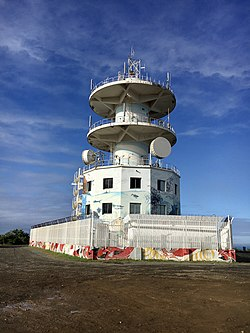
\includegraphics[width=0.2\textwidth]{ressources_rapport/tour_montravel.jpg}
    \caption{Tour Montravel inaugurée en 1995 à Nouméa, abritant les coeurs des réseaux fixe et mobile et assurait ainsi la couverture téléphonique des Nouméens.}
\end{figure}
\newpage

\section{La section GLIA de l'OPT}
\begin{figure}[h] % h = here (placer l'image ici)
    \centering
    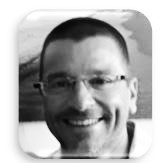
\includegraphics[width=0.2\textwidth]{ressources_rapport/adrien_sales.jpg}
\end{figure}
Lors du stage, j'ai travaillé au sein de la section GLIA (Génie Logiciel Inter-Applicatif) de l'OPT. Adrien SALES (chef de section) était mon maître de stage et commanditaire du projet renouvellement front-end. C'était avec lui que passait les échanges et retours sur le projet pour le travailler et l'améliorer au fur à mesure.

\cite{paroles_agent}

\vspace{1cm}
\begin{figure}[h] % h = here (placer l'image ici)
    \centering
    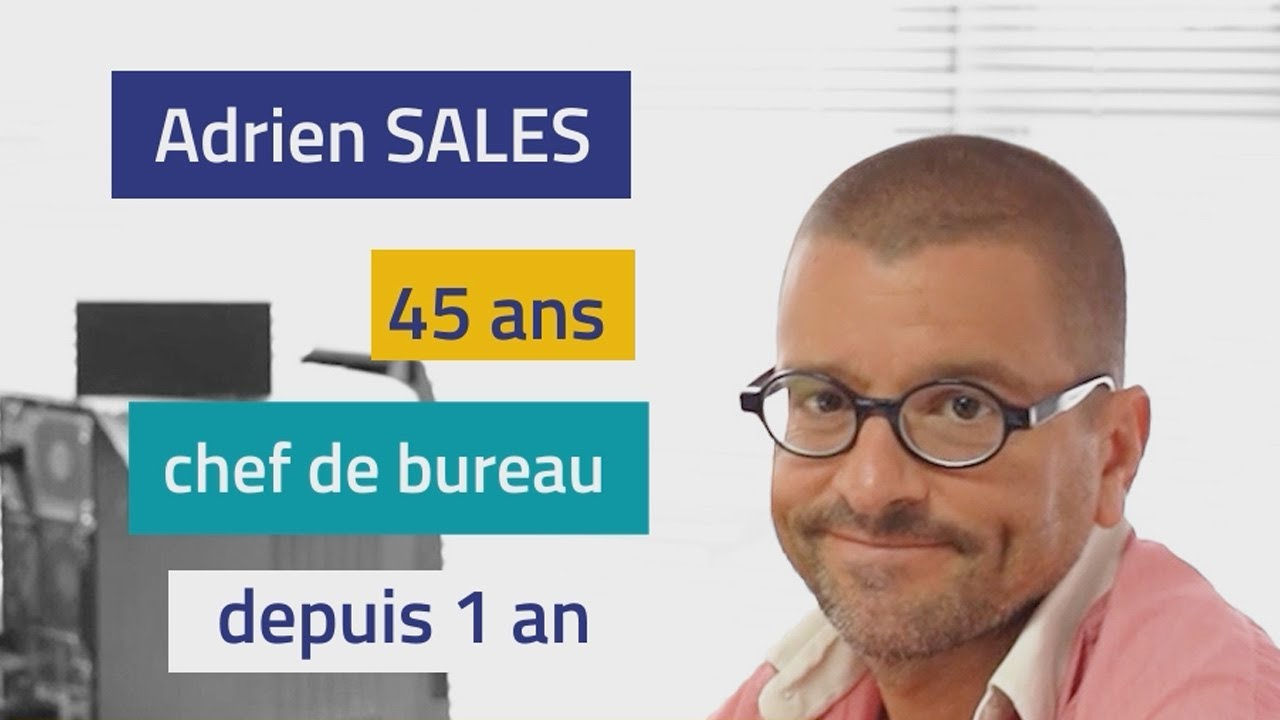
\includegraphics[width=0.4\textwidth]{ressources_rapport/paroles_agent.jpg}
    \caption{Miniature de "Paroles d'agent - Adrien SALES", qui a été publié le 19 février 2020 sur \href{https://www.youtube.com/watch?v=g2JuEcwPvgE}{https://www.youtube.com/watch?v=g2JuEcwPvgE}}
\end{figure}
Son rôle consiste à copier les données entre les différents systèmes de l'OPT-NC vers d'autres systèmes (exemple : prendre les données de télécommunications et les verser dans un autre endroit pour pouvoir les exploiter). afin que ces données puissent être utilisées en interne, notamment \cite{serie_articles} pour développer des solutions informatiques.
\newpage

\section{Etat des lieux de l'OPT : forces et faiblesses}
\begin{figure}[h] % h = here (placer l'image ici)
    \centering
    
\includegraphics[width=0.2\textwidth]{ressources_rapport/forces.png}
\end{figure}
Parmi les forces : 
\begin{itemize}
    \item Une omniprésence sur le territoire calédonien (plus de 50 agences).
    \item Une expertise technique interne pour offrir des solutions adaptées.
    \item Des infrastructures modernes pour recevoir les clients et leur proposer les services de l'OPT (Boîtes postales, Conseillers, Guichets automatique de billets, Guichets spécialisés).
\end{itemize}

\vspace{1cm}
\begin{figure}[h] % h = here (placer l'image ici)
    \centering
    
\includegraphics[width=0.2\textwidth]{ressources_rapport/faiblesses.png}
\end{figure}
Parmi les faiblesses : 
\begin{itemize}
    \item Certaines applications sont vieillissantes (comme la recherche d'agence OPT où certaines informations ne sont plus à jour et l'interface n'est plus ergonomique pour le standard de nos jours).
\end{itemize}

% =====================
\chapter{Renouvellement front-end de l'application web}
\section{Apprentissage des pré-requis (Next.js et GitHub)}
Avant d’entrer dans le développement de l'application, j’ai suivi une \cite{tuto_next} montée en compétence rapide sur Next.js, un framework open source s'appuyant sur la bibliothèque JavaScript React et sur la technologie Node.js. Ce framework est optimisé pour le rendu côté serveur et l’optimisation SEO : 

\vspace{1cm}
\begin{figure}[h] % h = here (placer l'image ici)
    \centering
    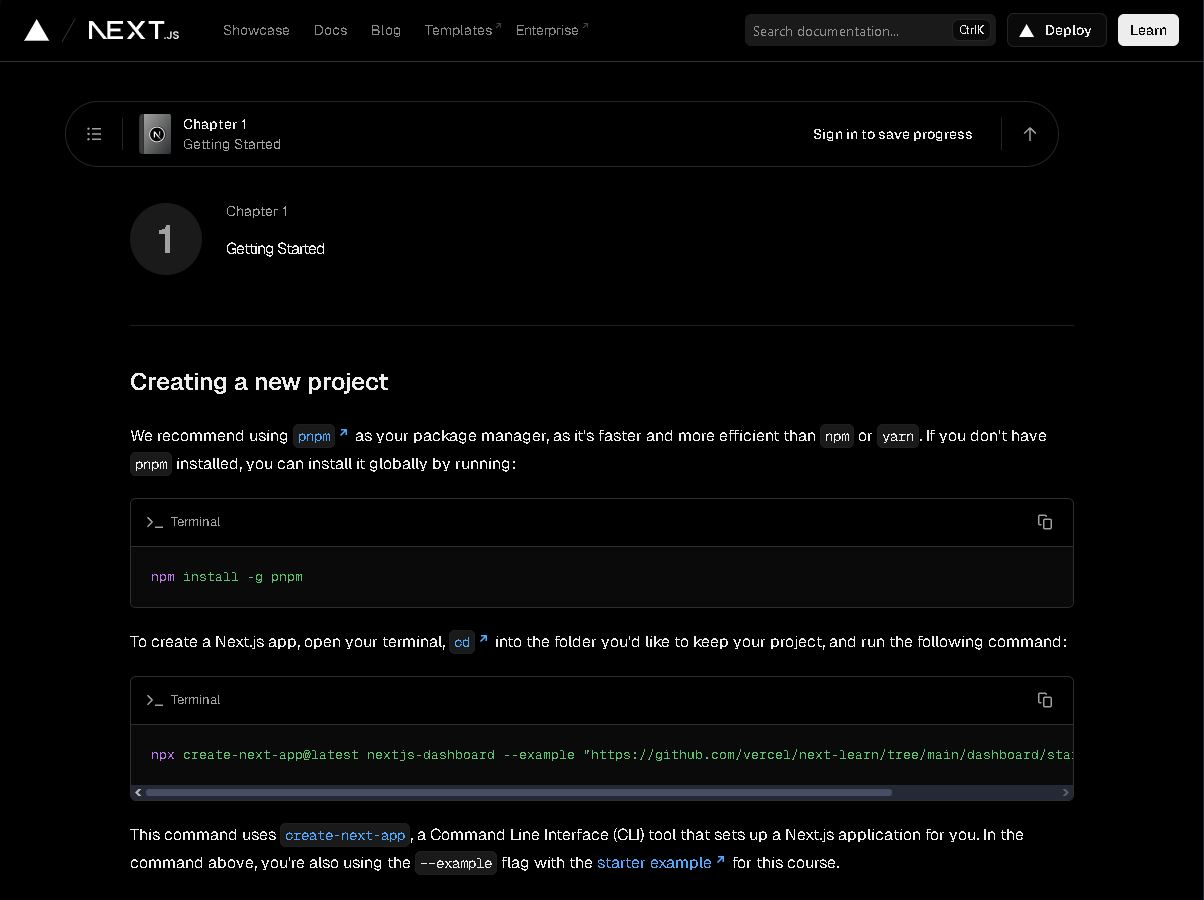
\includegraphics[width=0.7\textwidth]{ressources_rapport/learn_next.JPG}
    \caption{Screenshot du début du tutoriel aux bases de Next.js : \href{https://nextjs.org/learn/dashboard-app/getting-started}{https://nextjs.org/learn/dashboard-app/getting-started}}
\end{figure}

\vspace{1cm}
J’ai également pris en main GitHub pour versionner et collaborer efficacement avec Adrien SALES. Lorsqu'un de nous deux devait faire part d'un problème ou d'une suggestion par rapport au projet, on passait par les issues GitHub, et même parfois par des Pull Requests si il fallait review du code avant de le push sur la branche main de l'application. \cite{repo} La repo est publique : \href{https://github.com/adriens/unc-temps-attente-nextjs}{https://github.com/adriens/unc-temps-attente-nextjs}

\vspace{1cm}
\begin{figure}[h] % h = here (placer l'image ici)
    \centering
    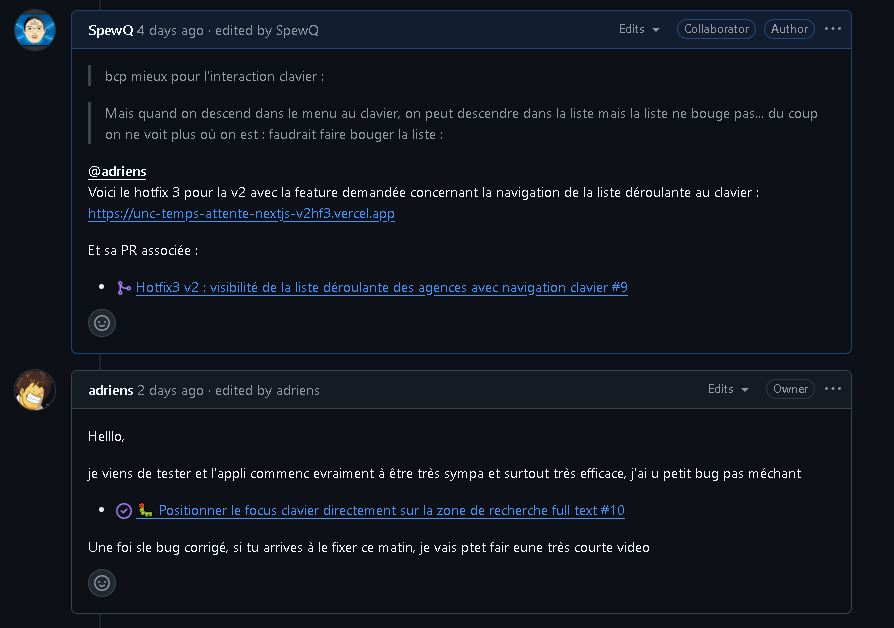
\includegraphics[width=0.7\textwidth]{ressources_rapport/extrait_issue_5.JPG}
    \caption{Extrait de l'issue 5 : Feedback sur la v2 de l'application}
\end{figure}

\begin{figure}[h] % h = here (placer l'image ici)
    \centering
    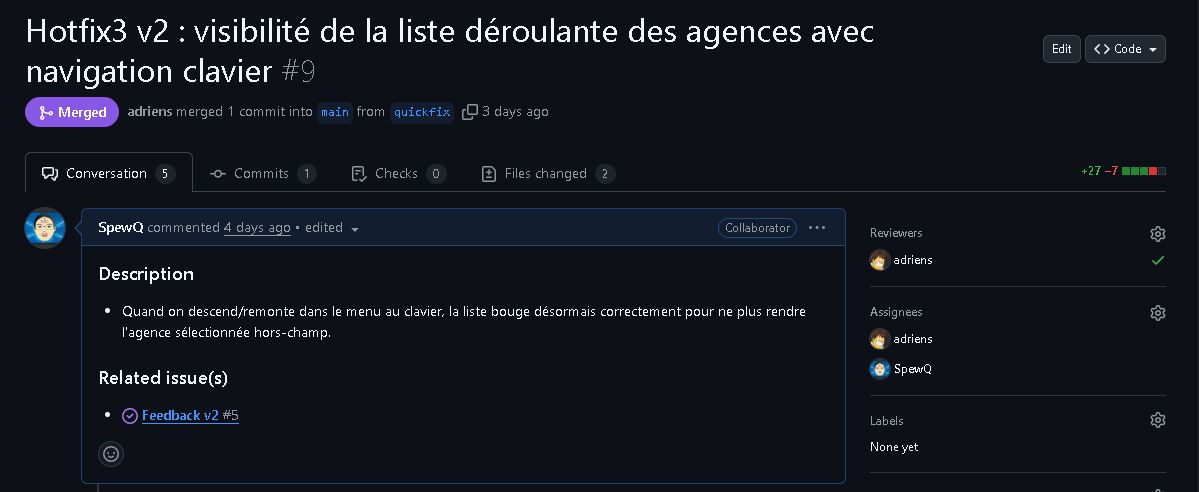
\includegraphics[width=0.7\textwidth]{ressources_rapport/extrait_pr_9.JPG}
    \caption{Extrait de la Pull Request 9 pour ajouter la fonctionnalité de voir la liste déroulante de la recherche d'agences sur navigation clavier}
\end{figure}
\newpage

\section{Propositions d'idées pour moderniser l'application}
En analysant l'application qui existait avant mon stage, voici ce que j'ai remarqué :
\begin{itemize}
    \item L'information prend du temps à être accédée. On doit scroller une sélection de communes pour cliquer sur une commune, et après rechercher la bonne agence en cliquant une deuxième fois, puis scroller les informations d'une agence.
\end{itemize}
\begin{figure}[h] % h = here (placer l'image ici)
    \centering
    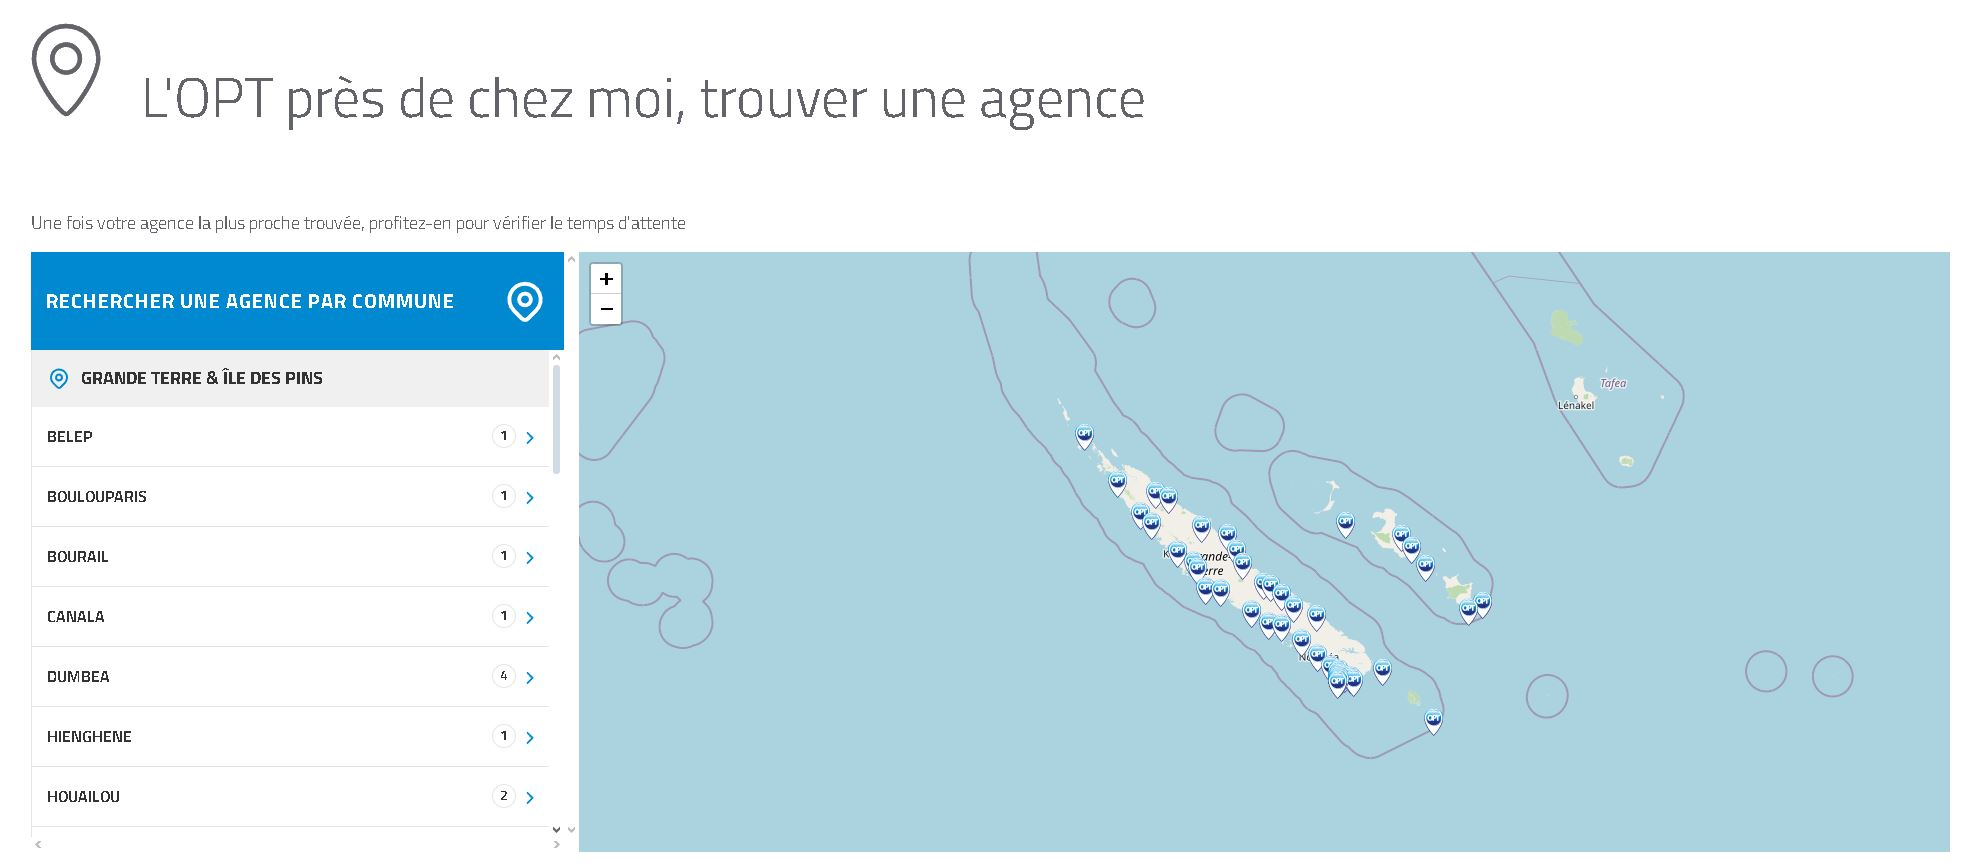
\includegraphics[width=1\textwidth]{ressources_rapport/ancien_app_opt.JPG}
    \caption{Ancienne application OPT Trouver une agence}
\end{figure}
\vspace{1cm}

\begin{figure}[h] % h = here (placer l'image ici)
    \centering
    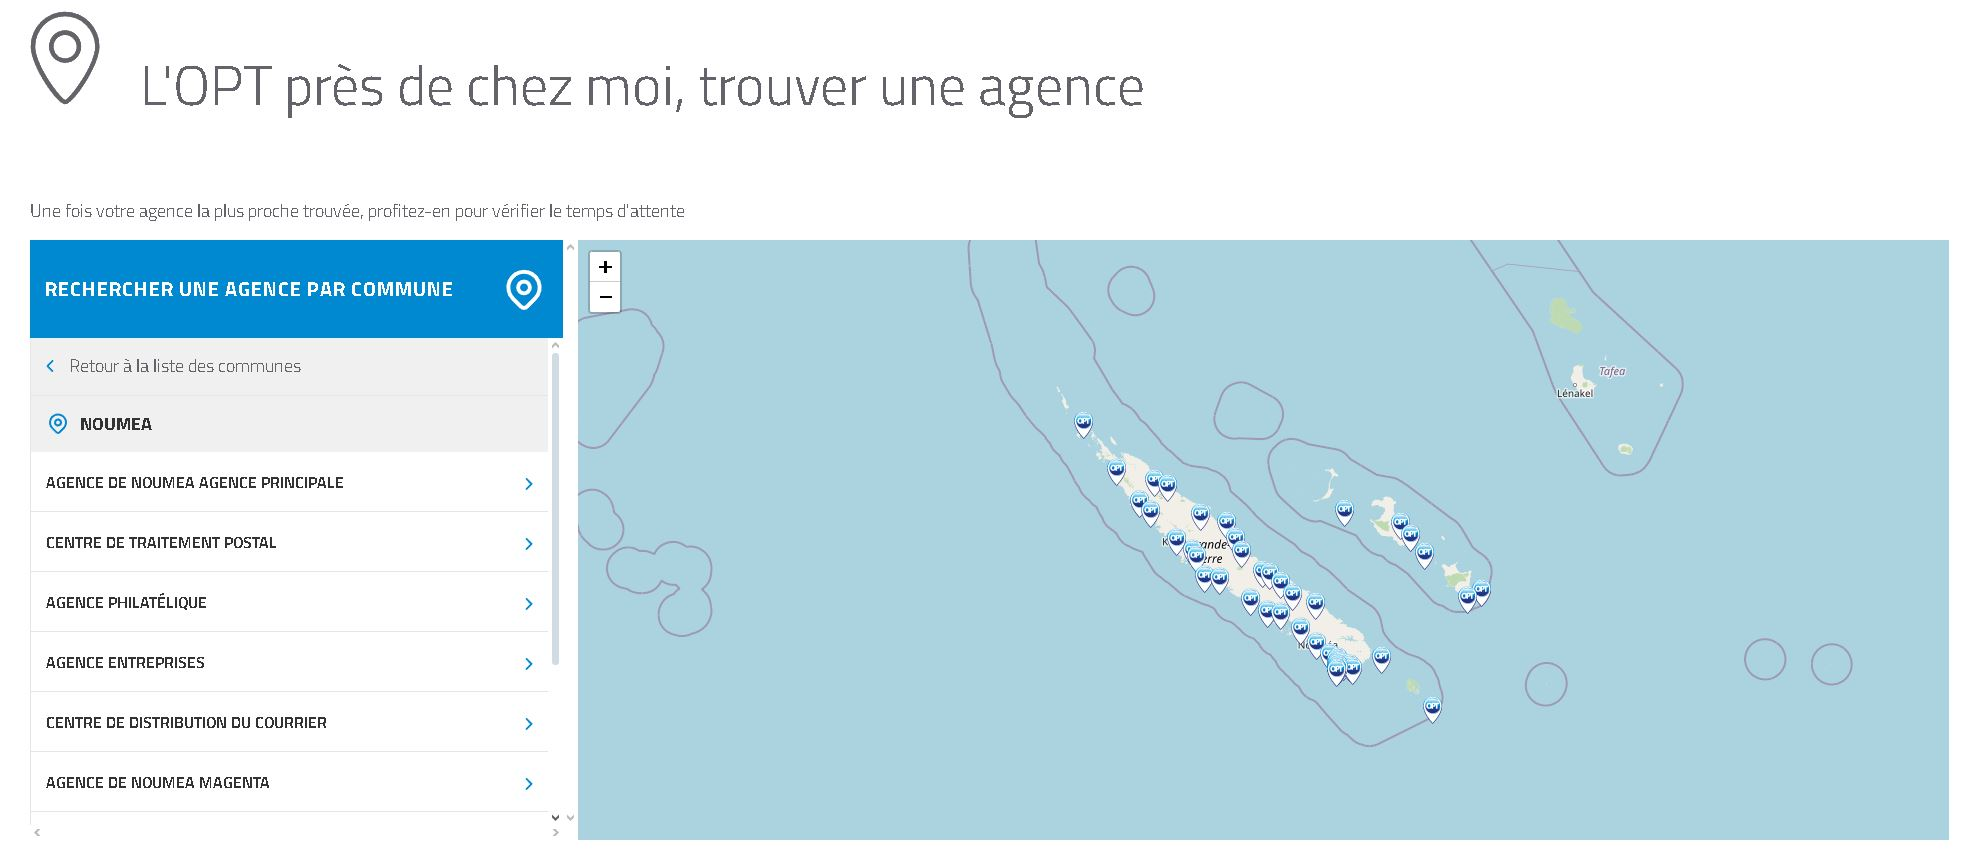
\includegraphics[width=1\textwidth]{ressources_rapport/ancien_app_opt_noumea.JPG}
    \caption{Nouméa sélectionnée}
\end{figure}
\vspace{1cm}

\begin{figure}[h] % h = here (placer l'image ici)
    \centering
    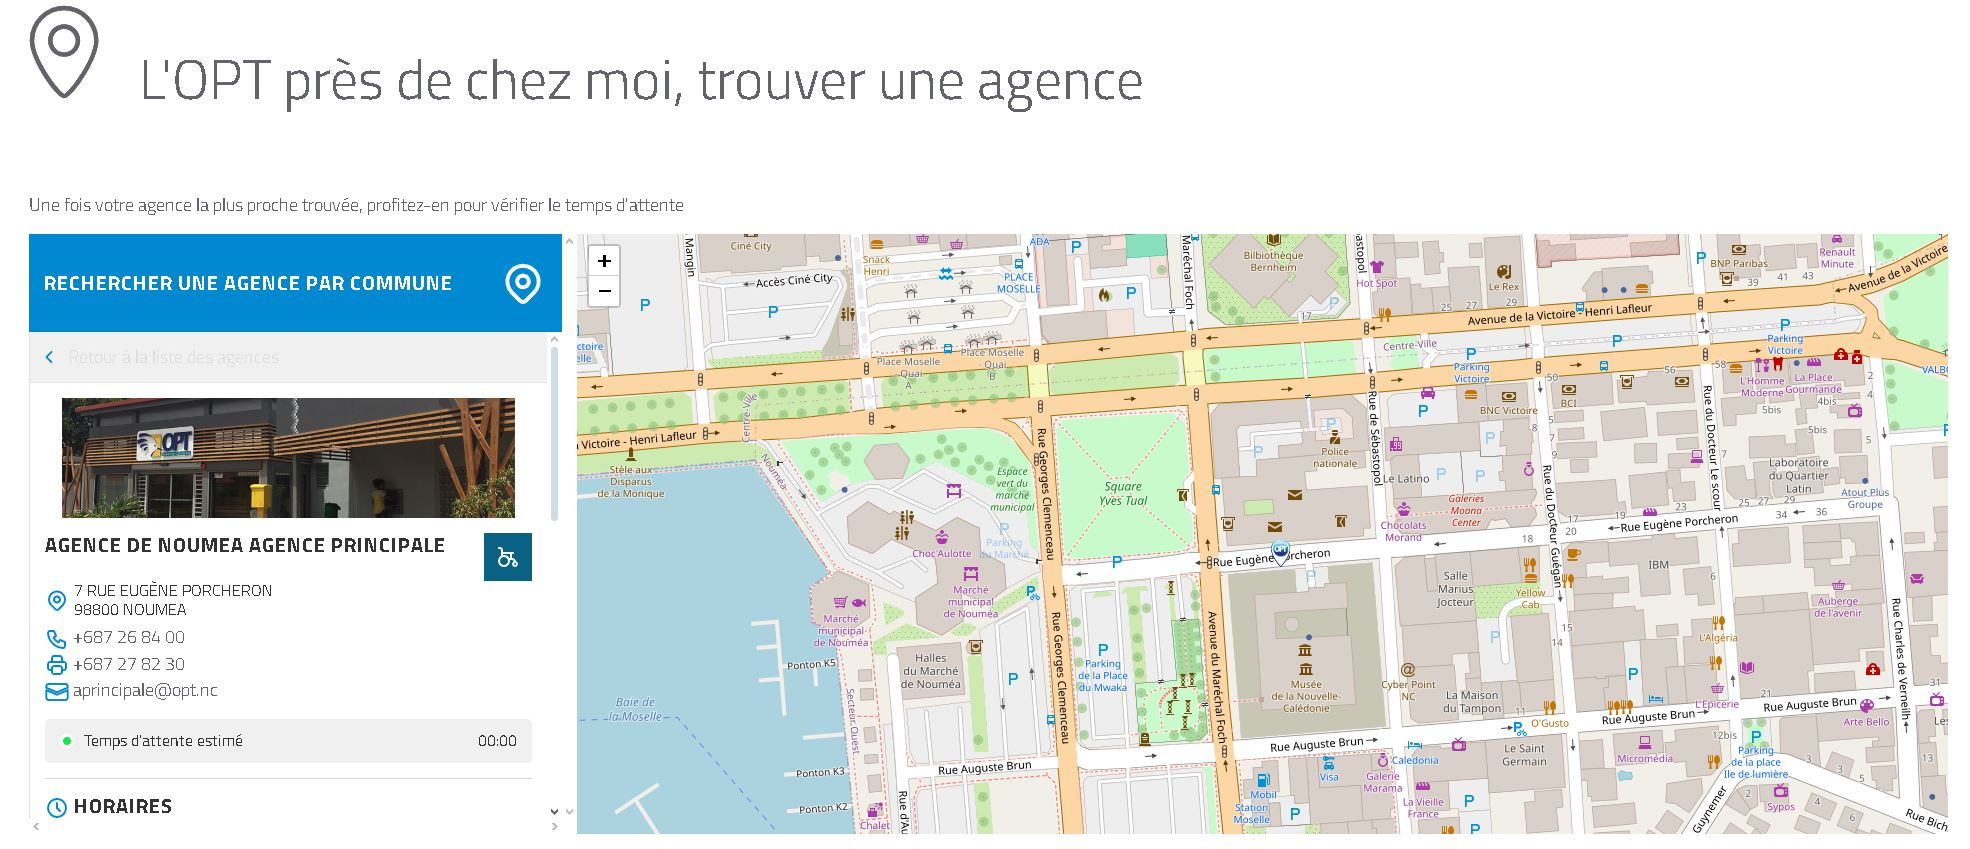
\includegraphics[width=1\textwidth]{ressources_rapport/ancien_app_opt_noumea_agence_principale.JPG}
    \caption{Agence principale sélectionnée}
\end{figure}
\vspace{2cm}
Suite à cette analyse, voici mes premières idées pour moderniser l'application :
\begin{itemize}
    \item Demander la position de l'utilisateur pour localiser l'agence la plus proche de celui-ci.
    \item La carte (sous React-Leaflet) sera centrée sur l'utilisateur au début pour faciliter ensuite la navigation autour.
    \item Repenser l'interface pour la rendre simple, fluide et ergonomique.
\end{itemize}

\newpage

\section{Pourquoi utiliser Next.js, Vercel et le portail d'API APIGEE de l'OPT}
Vu qu'il fallait que je modernise l'application pour qu'elle soit simple et fluide d'utilisation et que je puisse avoir du feedback dessus, Adrien SALES m'avait explicité d'utiliser ces 3 technologies :
\vspace{0.5cm}
\begin{itemize}
    \item \textbf{Next.js :} Ce framework basé sur React gère efficacement le rendu côté serveur, ce qui améliore considérablement le temps de chargement des pages et le référencement SEO. Next.js a également un système de routage basé sur le système de fichiers qui facilite la création de pages, ce qui permet au développeur de se concentrer sur l'UI et l'UX.
    \vspace{0.5cm}
    \item \textbf{Vercel :} Pour lancer la première version de l'application de manière simple et efficace, le \cite{deploy_vercel} déploiement sur Vercel est pertinent puisque c'est une plateforme cloud et gratuit nécessitant juste une configuration minimale et une repo GitHub. À chaque push sur la repo associée au projet Vercel, un déploiement s'effectue automatiquement pour que Adrien SALES puisse suivre l'avancée du projet et que j'obtienne ses retours. De plus, Vercel est vivement recommandé par le tutoriel Next.js : \href{https://nextjs.org/learn/pages-router/deploying-nextjs-app}{https://nextjs.org/learn/pages-router/deploying-nextjs-app}
    \vspace{0.5cm}
    \item \textbf{\href{https://apigee-optnc-prd-api.apigee.io}{Portail API APIGEE de l'OPT :}} \cite{comprendre_apigee} APIGEE est la plate-forme native de gestion des API de Google Cloud pour créer, gérer et sécuriser des API. Elle propose des proxys d'API afin de créer une interface fiable et mettre à disposition des APIs publiques. Pour afficher les agences, les positionner correctement sur la carte et récupérer certaines métadonnées pour les afficher à l'utilisateur, le sujet du stage disait de passer par le portail API public de l'OPT. Pour comprendre comment l'utiliser, je me suis appuyé sur cet \cite{apigee} article : \href{https://dev.to/optnc/apigee-101-onboarding-authentication-1ghl}{https://dev.to/optnc/apigee-101-onboarding-authentication-1ghl}
    \cite{apigee_yt} On crée un compte sur le portail, puis dans apps (en cliquant en haut à droite sur son e-mail), on crée une nouvelle application qui permettra de choisir quelles APIs peuvent être appelées, et générer une clé API pour autoriser le traitement de données nécessaire.
\end{itemize}
\vspace{0.5cm}
Ces trois technologies sont parfaites pour le stage, car elles couvrent la chaîne de développement et production de l'application. Next.js et APIGEE permettent de récupérer les données en temps réel et de les afficher sous forme de carte interactive dans une interface moderne et performante, et Vercel est idéale pour un stage car elle met cette interface à disposition grâce un flux de déploiement fluide depuis GitHub.

\newpage

\section{Développement et déploiement d'une première version}
Une première version a été développée et déployée sur un environnement de test Vercel : \href{https://unc-temps-attente-nextjs-v1.vercel.app}{https://unc-temps-attente-nextjs-v1.vercel.app}
Elle permettait déjà :
\begin{itemize}
    \item De localiser l’utilisateur puis d'afficher sa position par un point vert
    \item D’afficher les agences OPT les plus proches en centrant la carte sur l'utilisateur
    \item De consulter des métadonnées basiques
\end{itemize}

\begin{figure}[h] % h = here (placer l'image ici)
    \centering
    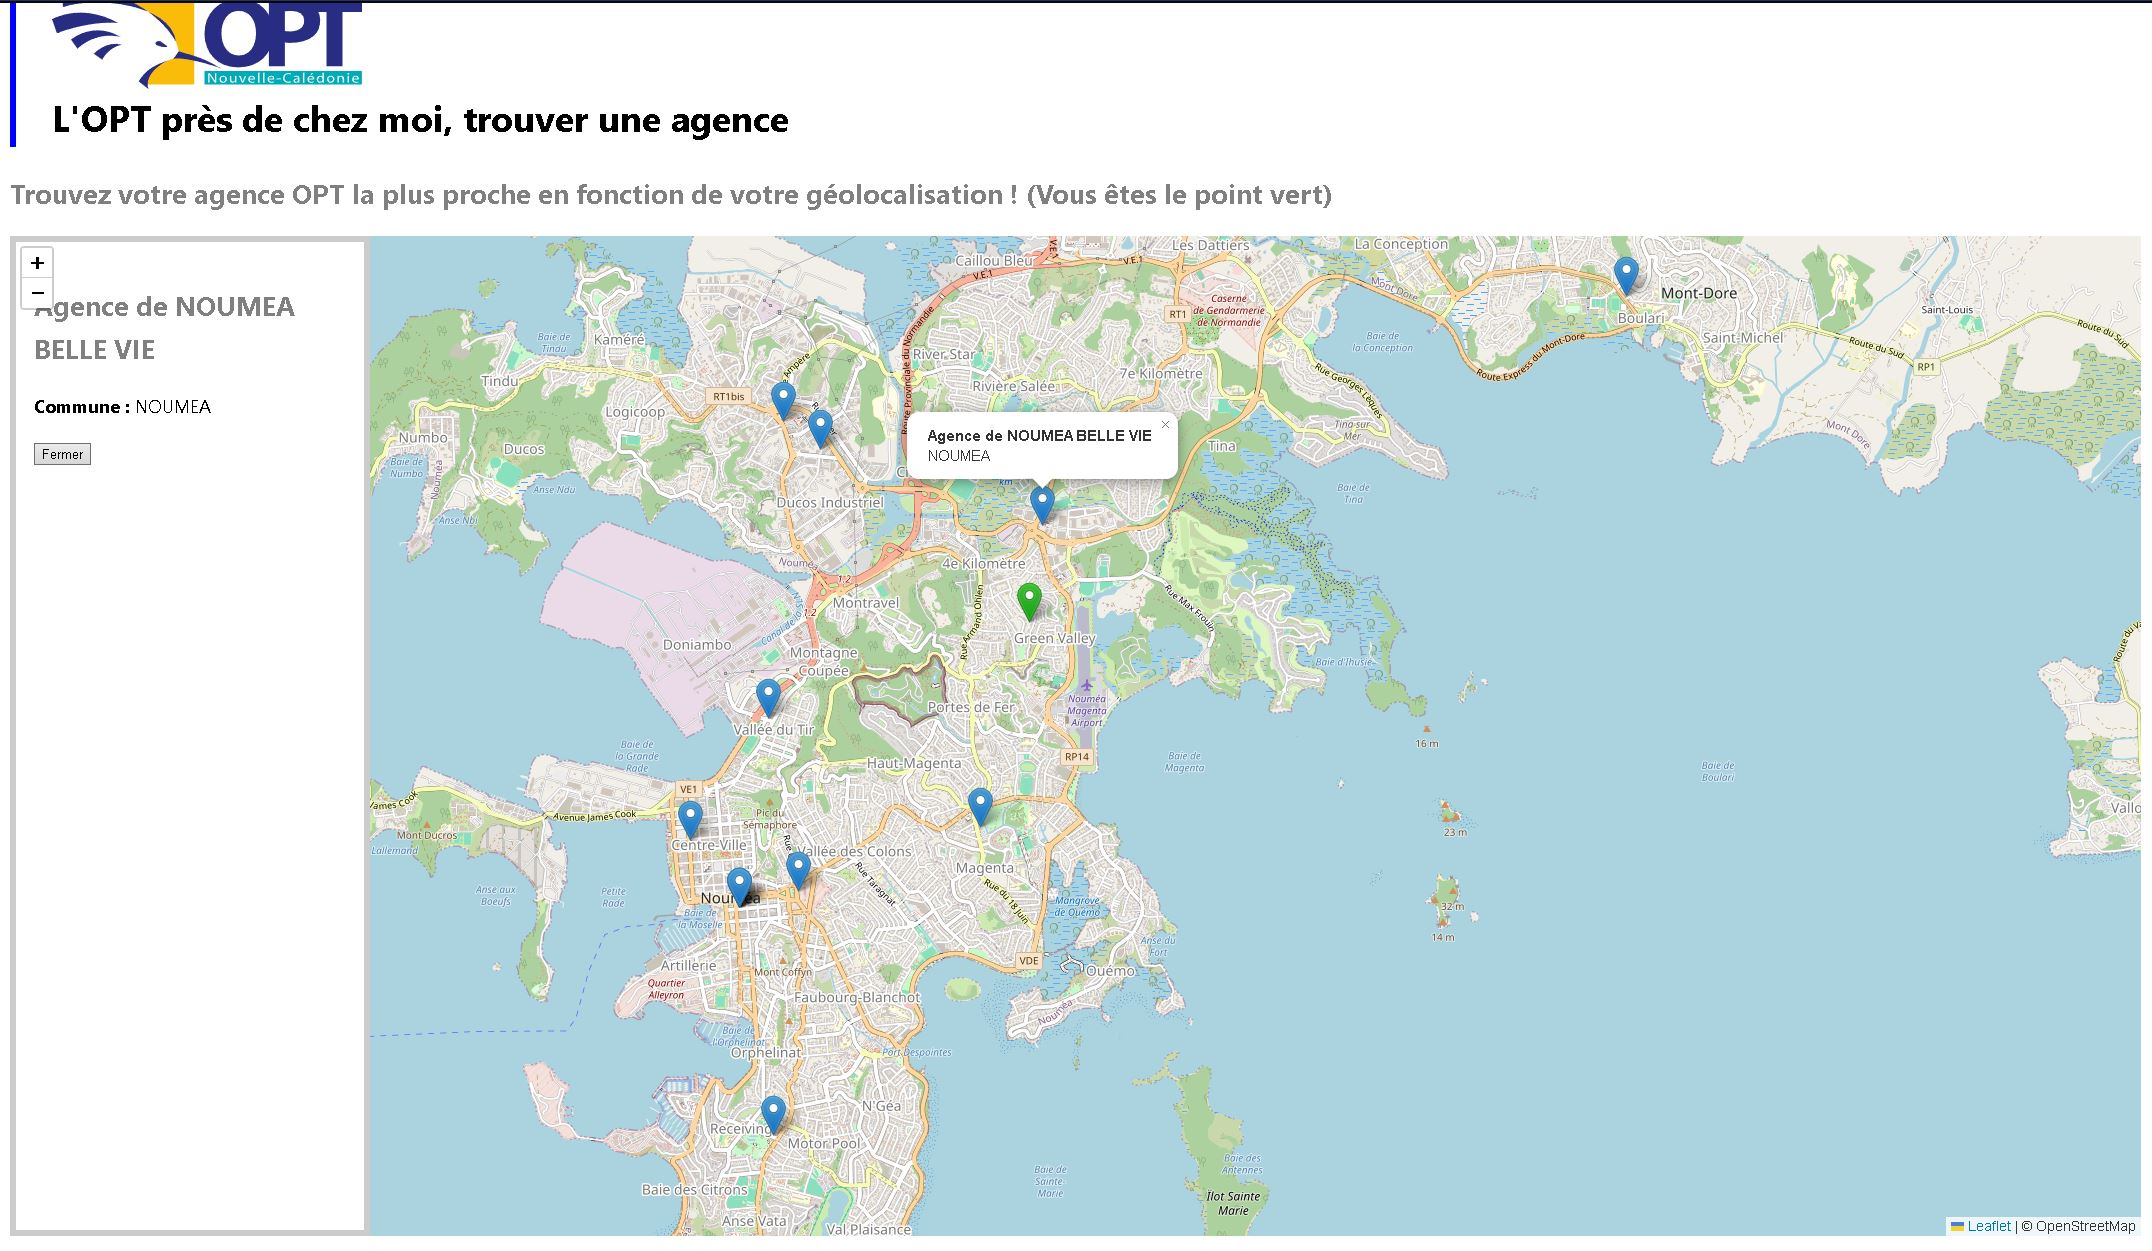
\includegraphics[width=1\textwidth]{ressources_rapport/app_opt_v1.JPG}
    \caption{v1 de l'application avec Agence Nouméa Belle-vie sélectionné}
\end{figure}
\vspace{1cm}
Suite au déploiement, je fais une demande de review  à Adrien SALES via une issue dédiée pour, afin de récolter du feedback sur cette v1 pour affiner l'application : \href{https://github.com/adriens/unc-temps-attente-nextjs/issues/4}{https://github.com/adriens/unc-temps-attente-nextjs/issues/4}

\begin{figure}[h] % h = here (placer l'image ici)
    \centering
    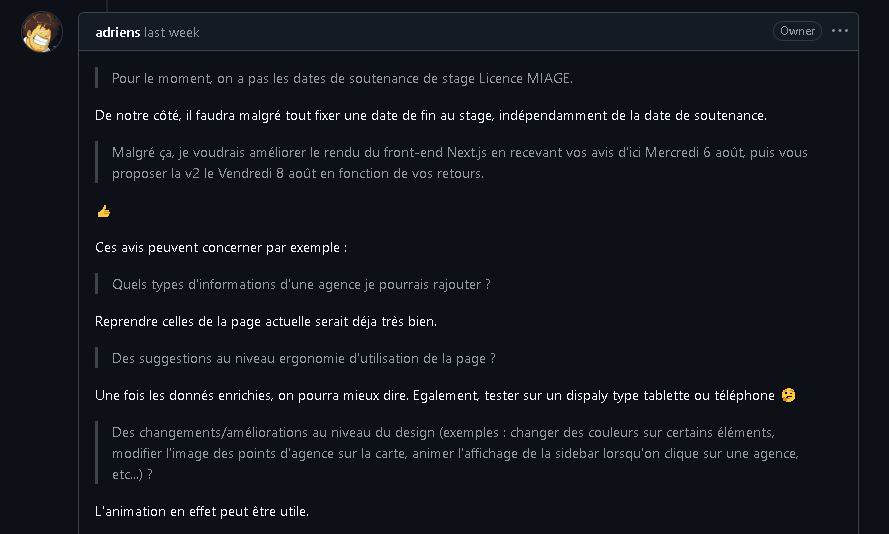
\includegraphics[width=1\textwidth]{ressources_rapport/extrait_issue_4.JPG}
    \caption{Extrait de l'issue 4 concernant le feedback de la v1}
\end{figure}
\newpage

\section{Répondre aux besoins du commanditaire par une deuxième version}
Après des échanges avec Adrien SALES sur la v1, la V2 (\href{https://unc-temps-attente-nextjs-v2.vercel.app}{https://unc-temps-attente-nextjs-v2.vercel.app}) a intégré :
\begin{itemize}
    \item Des métadonnées supplémentaires sur la sidebar pour enrichir les informations d'une agence (comme une adresse déduite par reverse geocoding).
    \item Une barre de recherche qui centre sur l'agence recherchée lorsqu'on la sélectionne.
\end{itemize}

\begin{figure}[h] % h = here (placer l'image ici)
    \centering
    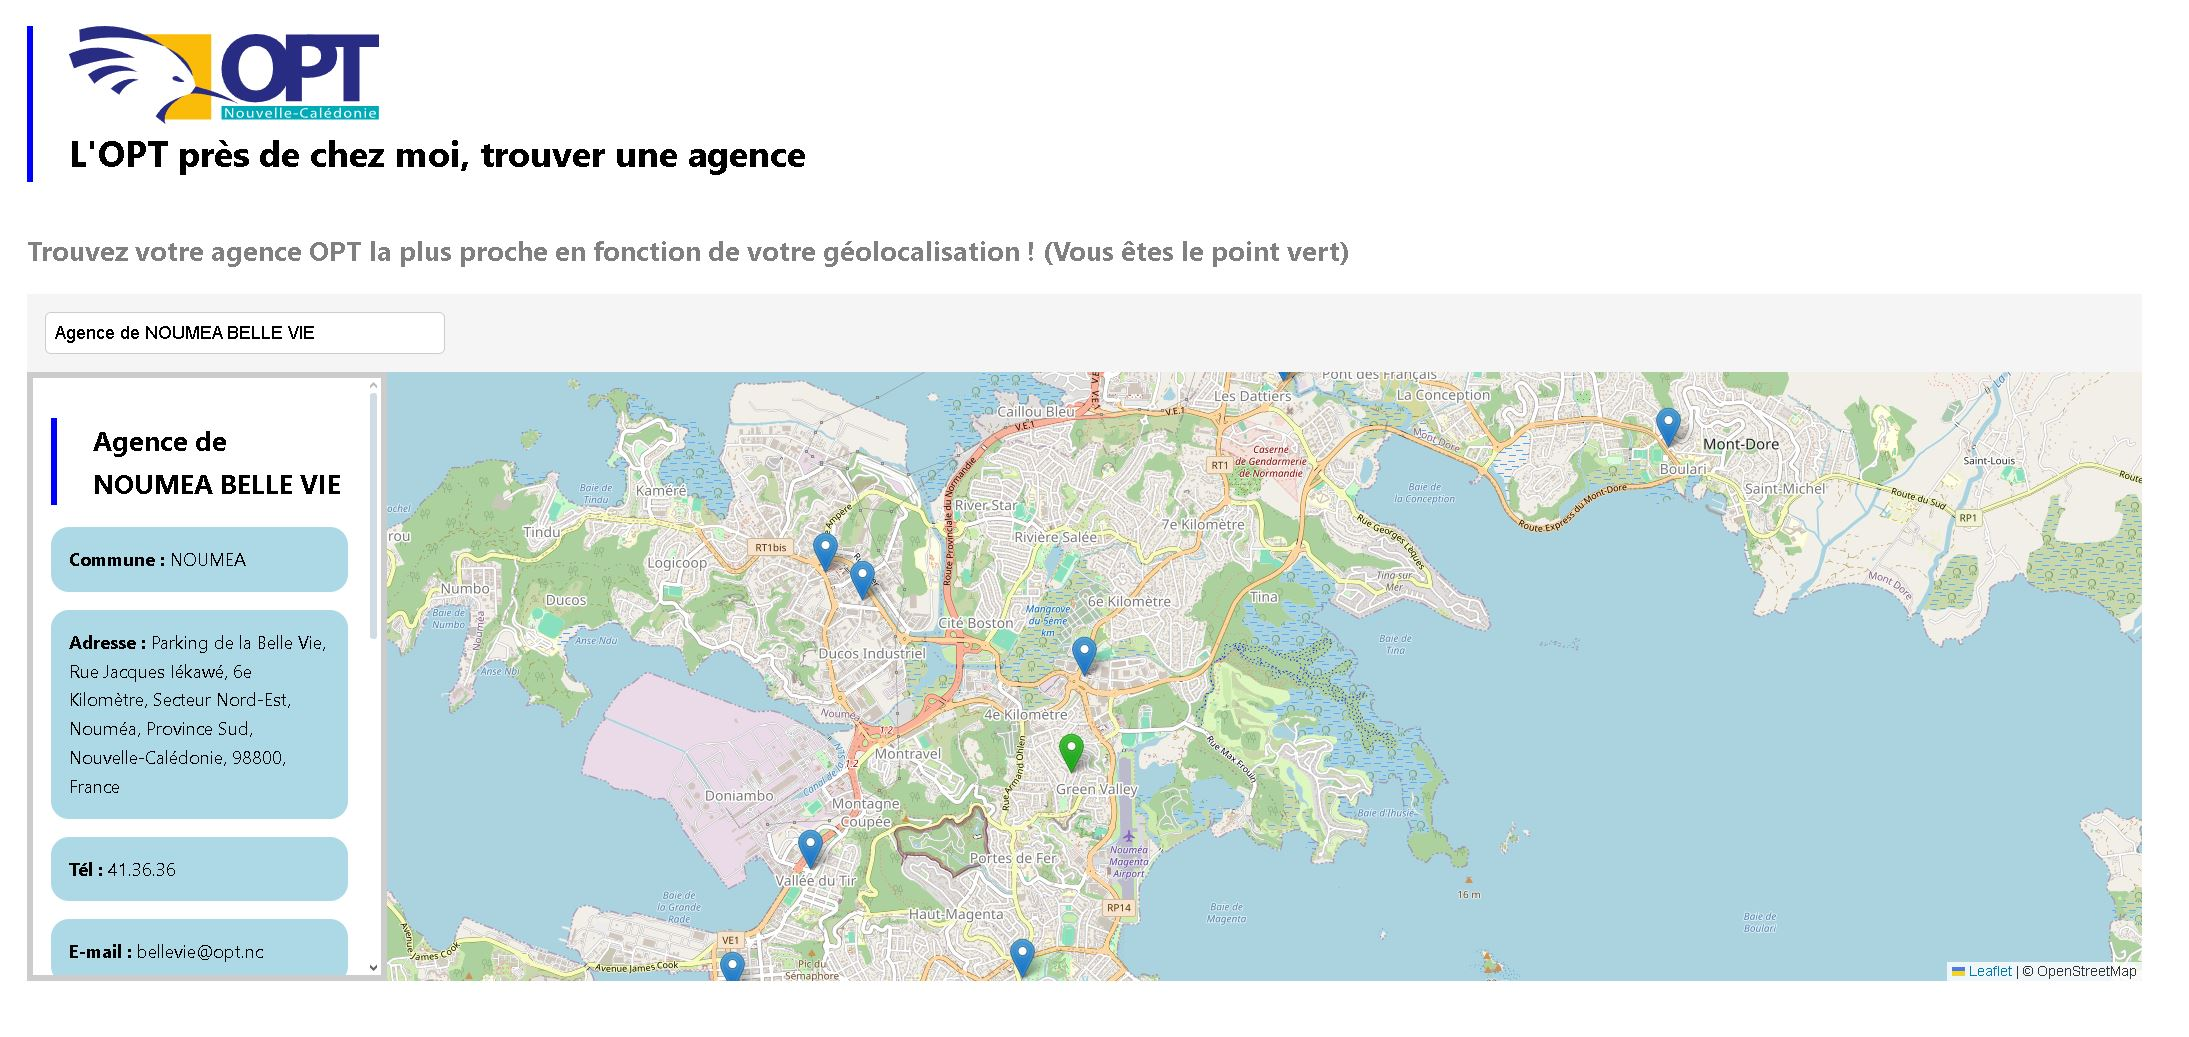
\includegraphics[width=1\textwidth]{ressources_rapport/app_opt_v2.JPG}
    \caption{v2 de l'application avec Agence Nouméa Belle-vie sélectionné}
\end{figure}
\vspace{8cm}
Donc comme pour la v1, j'ai créé une issue dédiée pour obtenir du feedback sur cette v2 : \href{https://github.com/adriens/unc-temps-attente-nextjs/issues/5}{https://github.com/adriens/unc-temps-attente-nextjs/issues/5}

\begin{figure}[h] % h = here (placer l'image ici)
    \centering
    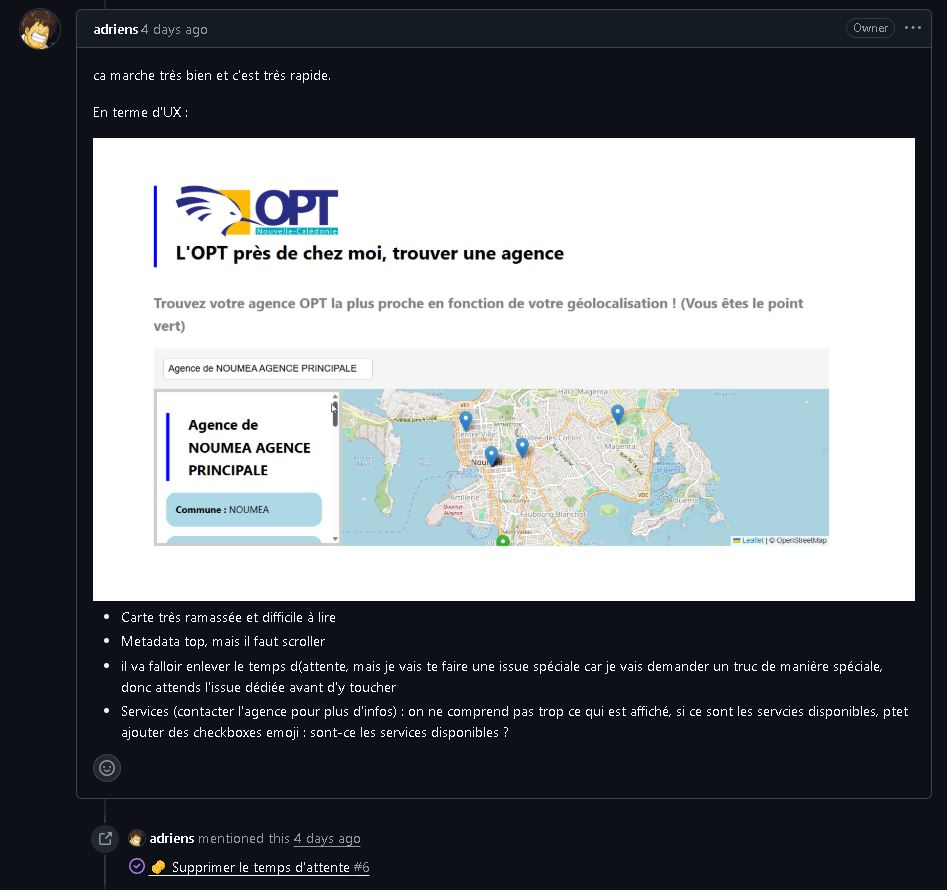
\includegraphics[width=0.5\textwidth]{ressources_rapport/extrait_issue_5_2.JPG}
    \caption{extrait de l'issue feedback v2 comportant de premiers retours (Revoir l'ergonomie de la carte et de la sidebar, expliciter la partie Services, enlever la partie temps d'attente}
\end{figure}
\newpage

\section{Peaufiner l'application pour un produit fini}
L'issue 5 consistait à des retours pour les implémenter sous forme de "hotfixes" car les suggestions ou les corrections étaient des petites améliorations pour ajuster correctement ce qu'on cherche à faire avec l'application : la recherche d'agence de manière simple et ergonomique : \href{https://github.com/adriens/unc-temps-attente-nextjs/pulls}{https://github.com/adriens/unc-temps-attente-nextjs/pulls}

\vspace{1cm}
Voici l'historique des hotfixes de cette v2 répertoriées dans les Pull Requests :
\vspace{1cm}

\begin{figure}[h] % h = here (placer l'image ici)
    \centering
    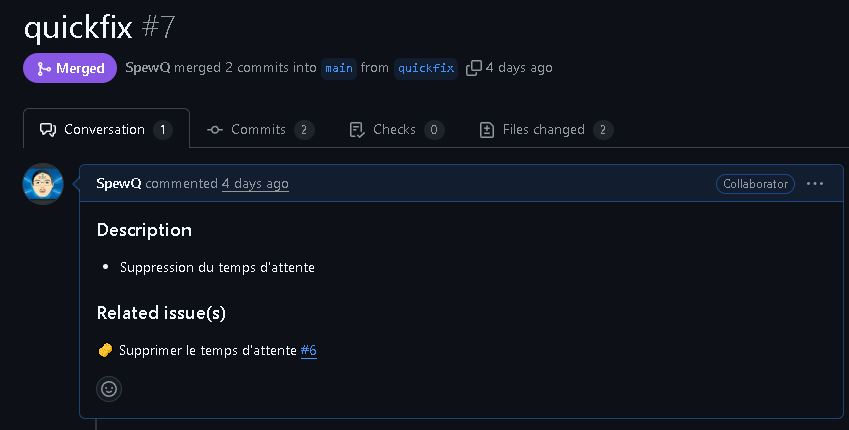
\includegraphics[width=0.7\textwidth]{ressources_rapport/extrait_pr_7.JPG}
    \caption{Hotfix 1 : supprimer la partie temps d'attente. \href{https://unc-temps-attente-nextjs-v2hf.vercel.app}{https://unc-temps-attente-nextjs-v2hf.vercel.app}}
\end{figure}

\begin{figure}[h] % h = here (placer l'image ici)
    \centering
    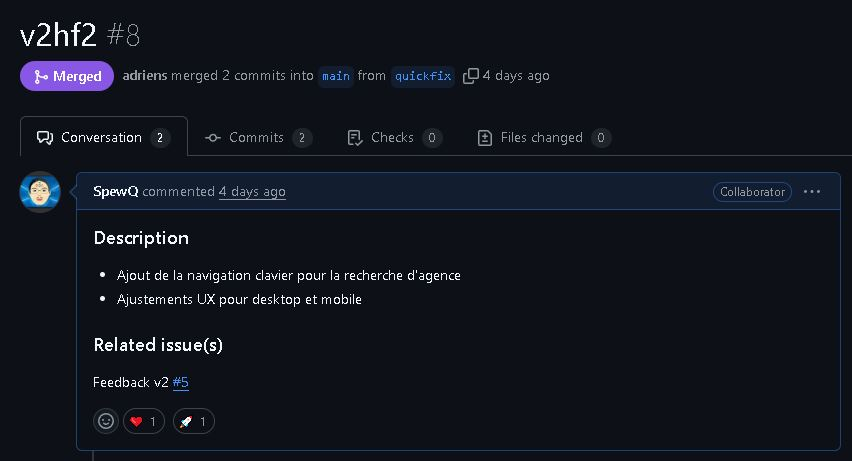
\includegraphics[width=0.7\textwidth]{ressources_rapport/extrait_pr_8.JPG}
    \caption{Hotfix 2 : ajout de la navigation clavier pour la recherche d'agence, et des ajustements UX pour desktop et mobile. \href{https://unc-temps-attente-nextjs-v2hf2.vercel.app}{https://unc-temps-attente-nextjs-v2hf2.vercel.app}}
\end{figure}

\begin{figure}[h] % h = here (placer l'image ici)
    \centering
    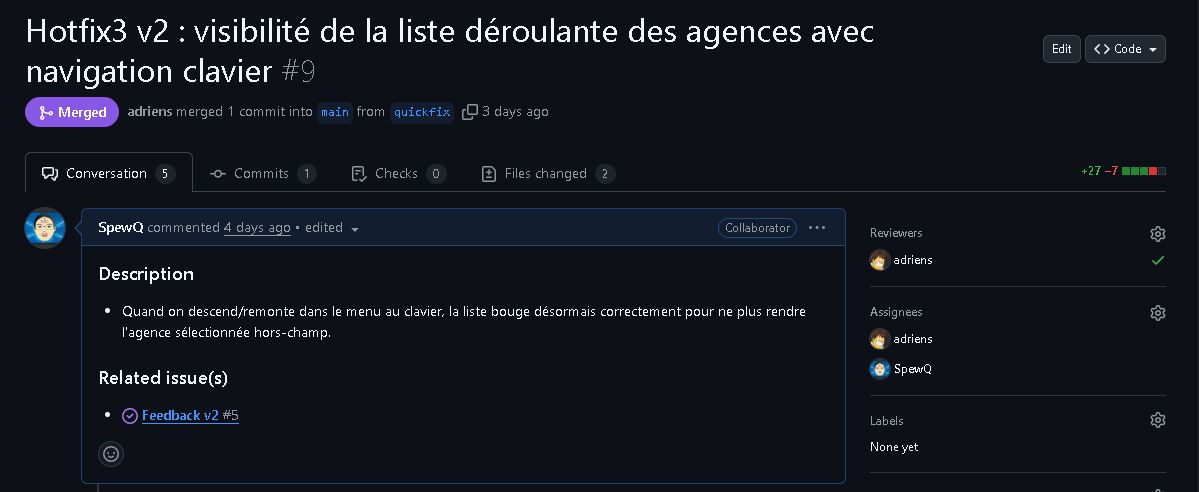
\includegraphics[width=0.7\textwidth]{ressources_rapport/extrait_pr_9.JPG}
    \caption{Hotfix 3 : Quand on descend/remonte dans le menu au clavier, la liste bouge désormais correctement pour ne plus rendre l'agence sélectionnée hors-champ. \href{https://unc-temps-attente-nextjs-v2hf3.vercel.app}{https://unc-temps-attente-nextjs-v2hf3.vercel.app}}
\end{figure}

\begin{figure}[h] % h = here (placer l'image ici)
    \centering
    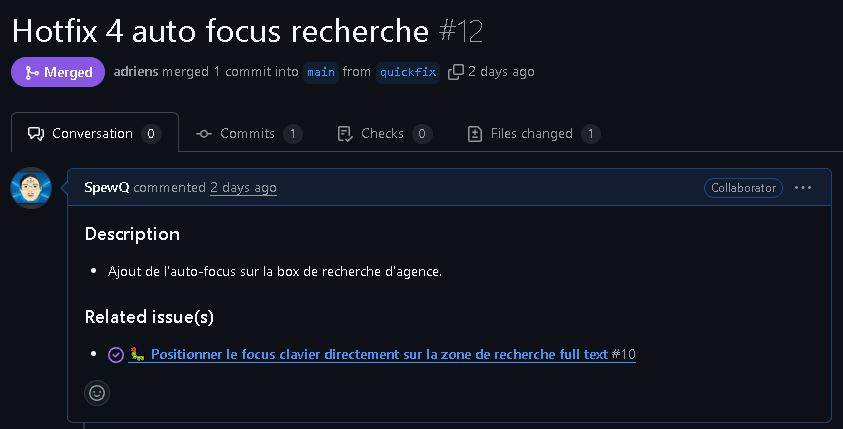
\includegraphics[width=0.7\textwidth]{ressources_rapport/extrait_pr_12.JPG}
    \caption{Hotfix 4 : Ajout de l'auto-focus sur la box de recherche d'agence. \href{https://unc-temps-attente-nextjs-v2hf4.vercel.app}{https://unc-temps-attente-nextjs-v2hf4.vercel.app}}
\end{figure}

% =====================
\chapter{Conclusion}
\section{Résultats du stage}
L’application \textit{"L'OPT près de chez moi, trouver une agence"} est désormais plus moderne, plus rapide et adaptée aux usages mobiles. Grâce à une optimisation UI et UX, les utilisateurs peuvent facilement trouver une agence avec la position utilisateur et la recherche d'agence pour consulter ses informations. Elle a une adresse URL clean où celle-ci sera up-to-date à chaque push sur la branche main de la repo GitHub de l'application : \href{https://unc-temps-attente-nextjs.vercel.app}{https://unc-temps-attente-nextjs.vercel.app}
\begin{figure}[h] % h = here (placer l'image ici)
    \centering
    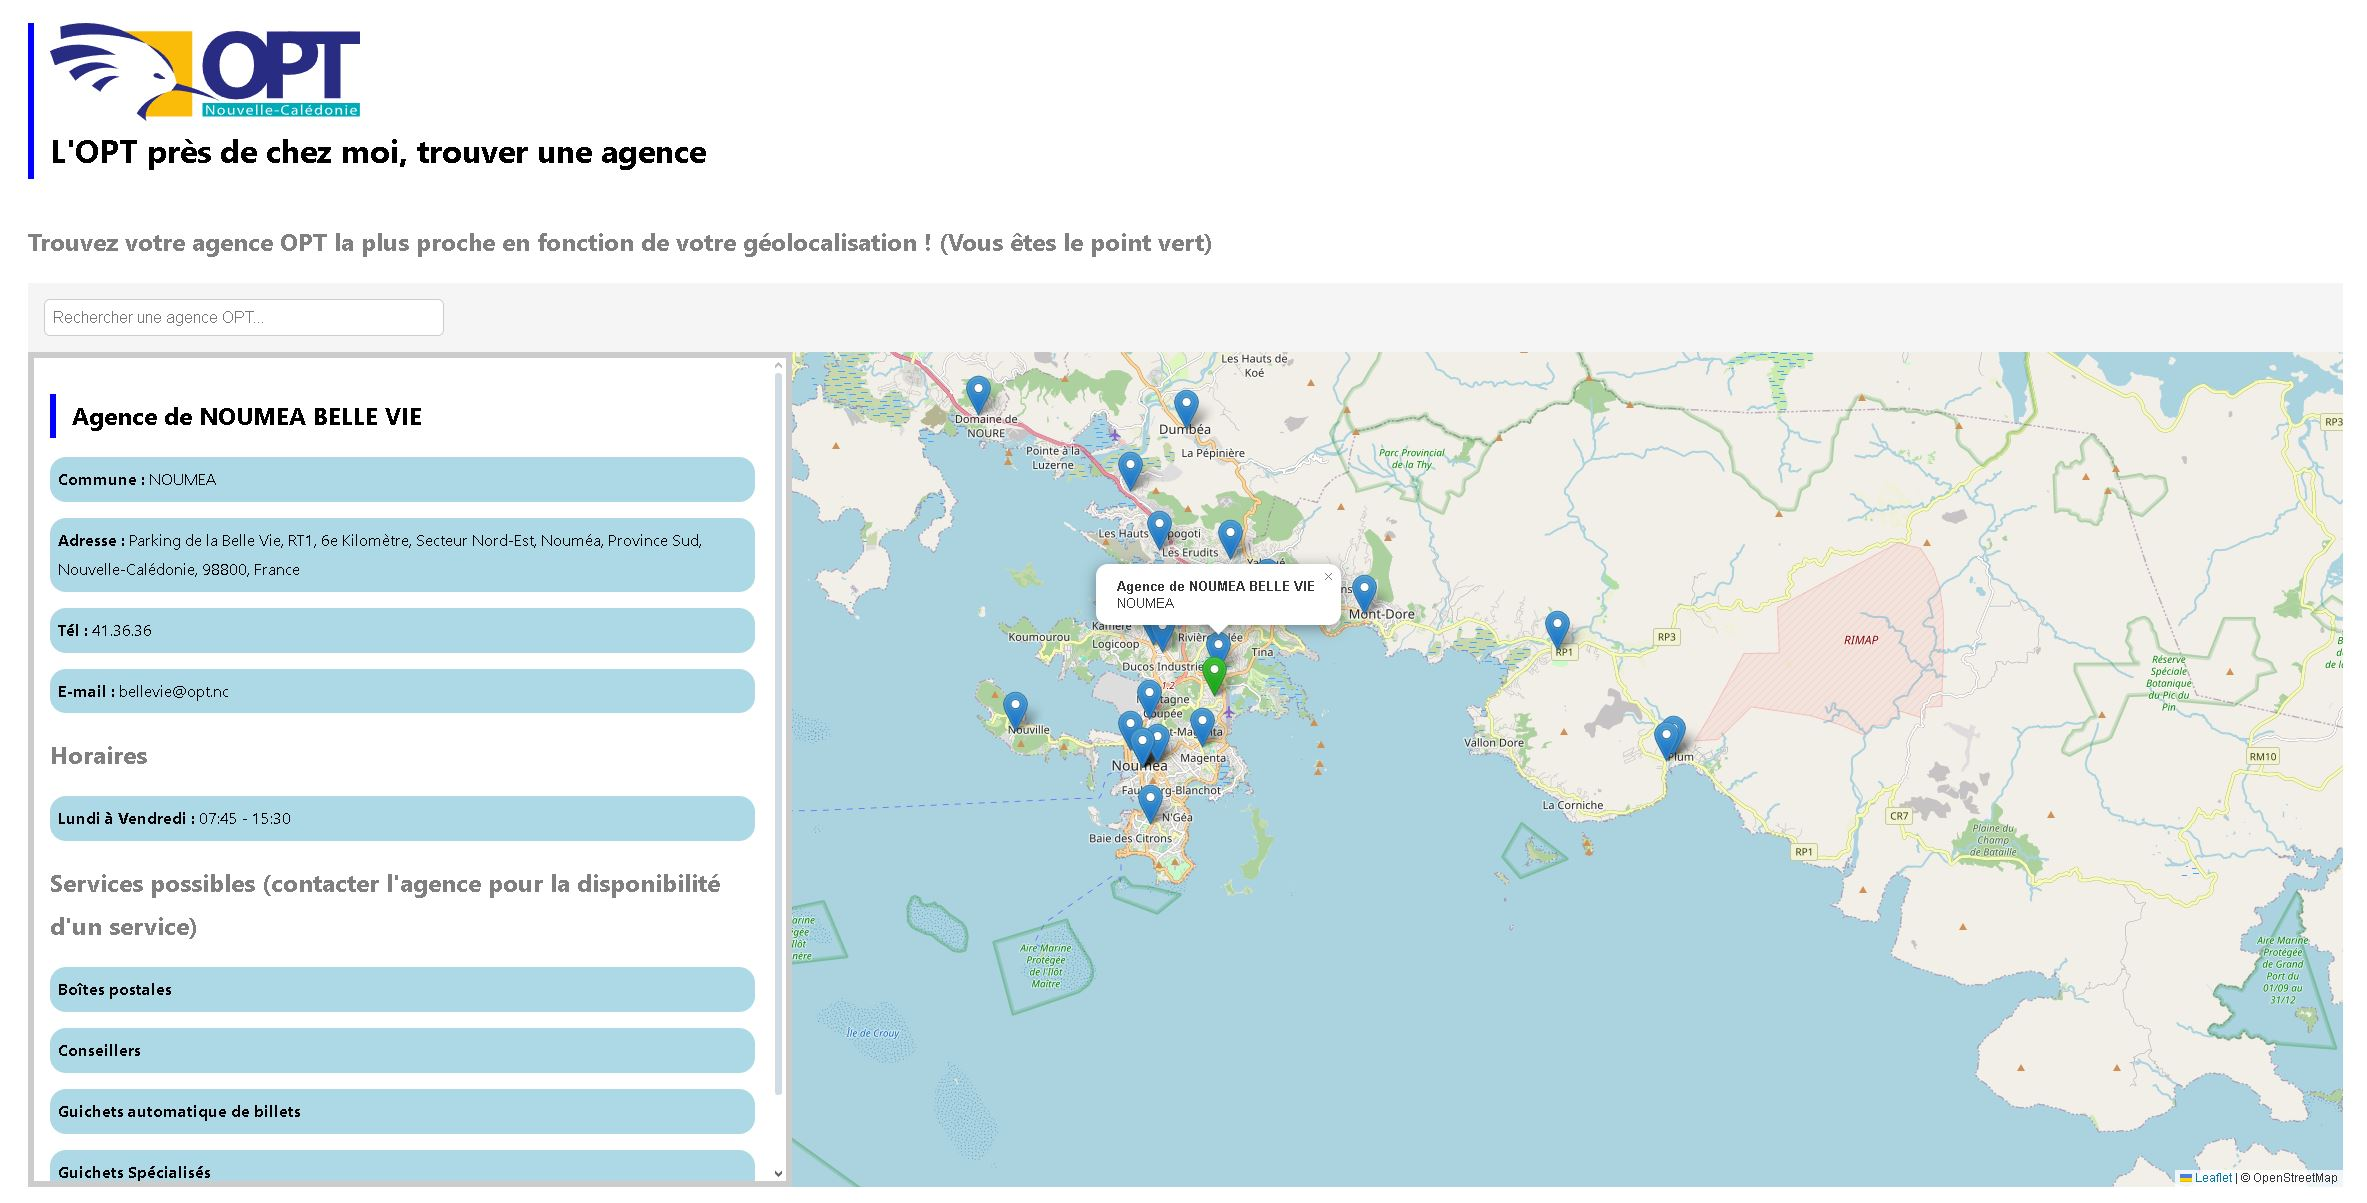
\includegraphics[width=1\textwidth]{ressources_rapport/app_opt.JPG}
    \caption{Rendu final de l'application web sous desktop à l'issue de ce stage.}
\end{figure}
\newpage

\section{Perspectives}
Les évolutions futures pourraient inclure :

\vspace{1cm}
\begin{figure}[h] % h = here (placer l'image ici)
    \centering
    
\includegraphics[width=0.2\textwidth]{ressources_rapport/temps_trajet.png}
    L’intégration des temps de trajet estimé d'une agence sélectionnée pour chaque mode de transport (à pied, en vélo, en voiture etc..).
\end{figure}

\vspace{1cm}
\begin{figure}[h] % h = here (placer l'image ici)
    \centering
    
\includegraphics[width=0.2\textwidth]{ressources_rapport/rdv.png}
    L’ajout d’un module de prise de rendez-vous en ligne.
\end{figure}

\vspace{1cm}
\begin{figure}[h] % h = here (placer l'image ici)
    \centering
    
\includegraphics[width=0.2\textwidth]{ressources_rapport/offline.png}
    Un mode hors ligne pour les zones à faible couverture.
\end{figure}

% =====================
\chapter{Glossaire}
\begin{description}
    \item[Next.js :] Framework React avec rendu côté serveur.
    \item[Leaflet :] Bibliothèque JavaScript pour cartes interactives.
    \item[Reverse Geocoding :] Conversion de coordonnées GPS en adresse lisible.
    \item[Vercel :] Plateforme de déploiement optimisée pour les projets JavaScript/React.
    \item[API :] Interface de programmation permettant à des applications de communiquer.
    \item[UI :] User Interface, l'interface utilisateur.
    \item[UX :] User Experience, l'expérience utilisateur qui comprend l'ergonomie d'utilisation d'une application.
    \item[Repo :] Terme utilisé pour un répertoire de projet GitHub.
    \item[SEO :] Search Engine Optimization, c'est l'ensemble des techniques qui permettent à une page web d'être mieux référencée parmi les résultats d'un moteur de recherche.
\end{description}
\newpage

% =====================
\renewcommand{\bibname}{Ressources}
\addcontentsline{toc}{chapter}{Ressources}
\begin{thebibliography}{9}

\bibitem{blog_opt}
Blog Dev.to de l'OPT-NC : 
\url{https://dev.to/optnc}
\vspace{0.5cm}

\bibitem{paroles_agent}
Vidéo YouTube, \textit{Paroles d'agent - Adrien SALES} :
\url{https://www.youtube.com/watch?v=g2JuEcwPvgE}
\vspace{0.5cm}

\bibitem{serie_articles}
Série d'articles Dev.to OPT, Adrien SALES :
\url{https://dev.to/adriens/series/18414}
\vspace{0.5cm}

\bibitem{tuto_next}
Tutoriel Next.js, \textit{Getting started} :
\url{https://nextjs.org/learn/dashboard-app/getting-started}
\vspace{0.5cm}

\bibitem{repo}
Répertoire GitHub public du projet :
\url{https://github.com/adriens/unc-temps-attente-nextjs}
\vspace{0.5cm}

\bibitem{deploy_vercel}
Tutoriel déploiement Vercel, Next.js,  \textit{Deploying Your Next.js App} :
\url{https://nextjs.org/learn/pages-router/deploying-nextjs-app}
\vspace{0.5cm}

\bibitem{comprendre_apigee}
Article Dev.to OPT, Adrien SALES,  \textit{Get started with Apigee Management} :
\url{https://dev.to/optnc/get-started-with-apigee-management-55dg}
\vspace{0.5cm}


\bibitem{apigee}
Article Dev.to OPT, Adrien SALES, \textit{APIGEE
101: onboarding and authentication} :
\url{https://dev.to/optnc/apigee-101-onboarding-authentication-1ghl}
\vspace{0.5cm}

\bibitem{apigee_yt}
Vidéo YouTube de l'article APIGEE
101: onboarding and authentication, \textit{APIGEE OPT - onboarding portail} :
\url{https://www.youtube.com/watch?v=L56z2Vkht5E}
\vspace{0.5cm}

\end{thebibliography}
\newpage

% =====================
% REMERCIEMENTS
\chapter*{Remerciements}
\addcontentsline{toc}{chapter}{Remerciements}

\begin{flushleft}
Je tiens à exprimer ma sincère gratitude à l'ensemble des personnes qui ont contribué au bon déroulement de mon stage et à l'élaboration de ce rapport.

\vspace{1cm}
Tout d’abord, je remercie \textbf{M. Loïc SALMON}, professeur tuteur à l’Université de la Nouvelle-Calédonie, pour son accompagnement, et m'avoir mis en contact avec l'OPT pour trouver le stage.

\vspace{1cm}
Mes remerciements s’adressent également à \textbf{Mme Claire LESCHI}, responsable pédagogique de la licence MIAGE, pour sa disponibilité et son implication dans l’encadrement global de notre formation.

\vspace{1cm}
Enfin, je souhaite également remercier chaleureusement \textbf{M. Adrien SALES}, mon maître de stage à l’OPT, pour son accueil, sa confiance et la qualité de ses orientations techniques, qui m’ont permis de progresser significativement sur le plan professionnel et personnel.
\end{flushleft}

\end{document}